\section{Data Center}

This section aims to provides an overview of the main architectural principles that underpin modern data centers. It is explored the separation between the physical and virtual network layers as well as how these components interact to deliver scalability and reliability in large-scale environments.

\subsection{Overview}
\paragraph{}
Data centers are physical facilities designed to house information systems and telecommunications equipment, as well as to process and distribute large volumes of data securely and efficiently. They integrate cooling systems, redundant power supplies and both physical and logical controls to ensure the continuous and reliable operation of organizations.\par

A data centers is generally divided into five main blocks. The first is the physical infrastructure, which encompasses racks, structured cabling, cooling systems, and fire detection and suppression systems. The second is data processing and storage, including both physical and virtualized servers, storage arrays, and associated systems. The third component is the network infrastructure, the key to operations, which interconnects the data center with external environments, such as cloud services or remote sites, comprising routers, firewalls and switches. The fourth component is the management system, responsible for event logging, continuous monitoring, and maintaining environmental stability. Finally, the fifth component corresponds to the security mechanisms, which protects data through physical and logical controls, including network segmentation (VLAN, VNI), access policies and encryption in transit and at rest. \par

The predominant network architecture in today's data centers is the leaf-spine IP mesh, which operates at Layer 3 of the OSI model. The underlay typically employs a high Maximum Transmission Unit (MTU) to support encapsulation overhead and relies on stable routing protocols, such as eBGP and OSPF. The overlay network is built atop this physical fabric, providing logical segmentation and workload mobility without IP addresses modification. Technologies such as VXLAN, NVGRE and Geneve are central to this virtualized architecture and will be examined in greater depth in subsequent sections.\par

\subsection{Data Center Network Architecture}
The foundation of modern data centers lies in the separation between the underlay, which represents the physical network infrastructure, and the overlay, which comprises the virtual networks. 
\newpage
\begin{wrapfigure}{r}{0.48\textwidth}
    \centering
    \vspace{-5pt}
    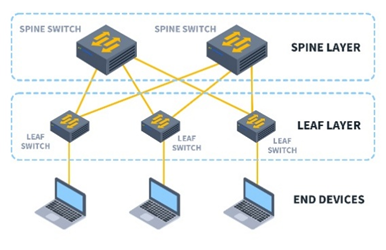
\includegraphics[width=0.9\linewidth]{Figures/LeafSpine.png}
    \caption{Leaf-spine structure.}
    \label{leafSpine}
\end{wrapfigure}

The underlay corresponds to the physical IP fabric of the network, typically organized in a Layer 3 leaf-spine topology. This topology, as illustrated in Figure \ref{leafSpine}, consists of two layers: the spine, formed by high-speed switches that constitute the network backbone; and the leaf, consisting of access switches that connect servers, storage devices and other endpoints. The primary objective of the underlay is to transport packets quickly and efficiently. For this reason, a high MTU, usually around 9000 bytes, is used to to accommodate encapsulation overhead and minimize fragmentation. 

The overlay is built on top of this fabric and consists of a set of virtual networks that encapsulate each user's traffic, providing logical isolation and mobility, without changing IP addresses. In practice, encapsulation mechanisms such as VXLAN, NVGRE or Geneve are employed. Each virtual network is identified by a unique segment ID, enabling scalable segmentation within large infrastructures. The central component of the overlay is the VXLAN Tunnel Endpoint (VTEP), typically residing on a leaf switch, responsible for encapsulating and decapsulating traffic between the overlay and the IP underlay. These virtual networks are often integrated with orchestration and automation platforms, which facilitate dynamic provisioning, policy enforcement and scalability. 

Correct MTU configuration within the underlay is critical, as an insufficient MTU will result in packet packet fragmentation and drops. Therefore, it is essential to maintain a adequately large MTUs and continuously monitor fragmentation and transmission metrics. The use of UDP-based encapsulation enhances multiple available paths through Equal-Cost Multi-Path (ECMP) routing, improving flow distribution, maximizing the inherent parallelism of the leaf-spine architecture and improving overall network efficiency. \par

\subsection{Data Centers Virtualization}

\begin{wrapfigure}{r}{0.48\textwidth}
    \centering
    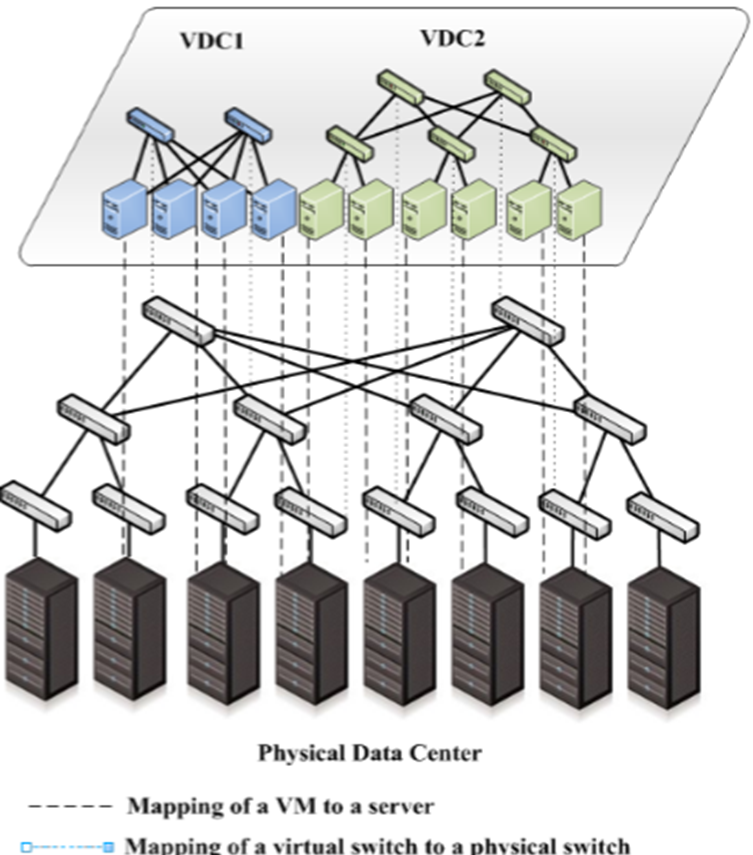
\includegraphics[width=0.8\linewidth]{Figures/virtualization.png}
    \caption{Virtualization of a Data Center.}
    \label{virtualization}
\end{wrapfigure}

A Virtualized Data Center (VDC) is a data center where some or all the hardware components, such as servers, routers, switches and network links, are virtualized. Typically, a physical hardware is virtualized using software or firmware known as hypervisor, which divides the equipment into multiple isolated and independent virtual instances. 

A VDC is defined as a collection of virtual resources, including VMs, virtual switches, and virtual routers, connected via virtual links and therefore constitutes a segment of a Virtual Data Center. While a Virtualized Data Center is a physical data center with deployed resource virtualization techniques, a Virtual Data Center is a logical instance of a Virtualized Data Center consisting of a subset of the physical data center resources. 

A Virtual Network (VN) is a set of virtual networking resources, such as virtual nodes (end-hosts, switches, routers) and virtual links and therefore, a VN is a part of a VDC. A network virtualization level is one of the layers of the network stack (application to physical) in which the virtualization is introduced. Figure \ref{virtualization}, shows how several VDCs can be deployed over a virtualized data center. 
